% vim: filetype=tex spell

\tikzstyle{winLbl} = [rectangle,text width=5em,text centered]

\newcommand{\cubesatonly}[2]{
    \draw (#1:#2) node{\pgftext[rotate=#1]{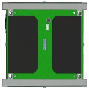
\includegraphics[height=\ARCheight]{cube-icon}}};
}

\newcommand{\biaswindow}[3]{%start,end,color
    \begin{scope}
        \clip                        (0,0)  -- (#1:\winR) arc (#1:#2:\winR) -- cycle;
        \draw[#3,thick]              (0,0)  -- (#1:\winR) arc (#1:#2:\winR) -- cycle;
        \fill[nearly transparent,#3] (0,0)  -- (#1:\winR) arc (#1:#2:\winR) -- cycle;
    \end{scope}
}

%digram showing bias windows for the alignment algorithm

\begin{tikzpicture}


    \def\incline{90}                            % Orbit Inclination (degrees)
    \def\poleWindow{10}                         % Polar alignment windows in degrees
    \def\offset{10}                             % Amount the window is offset in the wake direction (i.e.  earlier) in degrees eq_window = 15;
    \def\eqWindow{15}                           % Equatorial alignment window in degrees
    %\def\latTrigger{\incline-\poleWindow}       % Corrects polar window for inclination angle
    \def\latTrigger{80}                         % Corrects polar window for inclination angle
    \def\ARCheight{7mm}

    \def\winR{3cm}                                %window radius for drawing
    \def\axisLen{4cm}

    %import earth background
    \pgftext{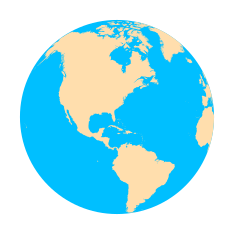
\includegraphics[height=4cm]{earth}}

    %draw orbit
    \draw[->,black,thin] (0,0) circle (\winR);

    %draw axis
    \draw[<->] (-\axisLen,0) -- (\axisLen,0);
    \draw[<->] (0,-\axisLen) -- (0,\axisLen);

    \draw[-{Triangle[width=6pt,length=6pt]}] (25:\winR+0.5cm) arc (25:45:\winR+0.5cm);
    \draw[winLbl]   (35:\winR+0.5cm) node[anchor=south west] {\small Orbit Direction};


    %draw bias windows
    %northbound equatorial window
    \biaswindow{\eqWindow/2 - \offset}{-\eqWindow/2 - \offset}{green}

    \draw[green,winLbl] (-\offset:\winR+0.5cm) node[anchor=north west] {\small Northbound Equatorial Window};
    %draw CubeSat
    \cubesatonly{-\offset}{\winR}


    %south bound equatorial window
    \biaswindow{180-\eqWindow/2 - \offset}{180 +\eqWindow/2 - \offset}{red}

    \draw[red,winLbl] (180-\offset:\winR+0.5cm) node[anchor=south east] {\small Southbound Equatorial Window};
    %draw CubeSat
    \cubesatonly{180-\offset}{\winR}


    %north polar window
    \biaswindow{\latTrigger - \offset}{90}{blue}

    \draw[blue,winLbl] (90-\poleWindow/2-\offset/2:\winR+0.5cm) node[anchor=south west] {\small North Polar Window};
    %draw CubeSat
    \cubesatonly{90-\poleWindow/2-\offset/2}{\winR}

    %draw axis labels
    \draw (0,\axisLen) node[anchor=south] {N};
    \draw (\axisLen,0) node[anchor=west] {E};

    \draw (0,-\axisLen) node[anchor=north] {S};
    \draw (-\axisLen,0) node[anchor=east] {W};

\end{tikzpicture}
